\chapter{System design and implementation}

\section{Overall architecture}

The system consists of five parts: editor plugin, resource model, execution system, debug bridge and test game. The editor plugin runs inside the Godot editor and is responsible for displaying behaviour tree resources as an operable GraphEdit canvas. The resource model stores nodes, parent-child relationships, Decorators, blackboard Schema and node coordinates. The execution system reads the same resource and passes Tick results to the game Actor. The debug bridge sends the current state, failure reasons and blackboard values back to the editor.

\begin{figure}[htbp]
\centering

\includegraphics[width=0.92\textwidth,height=0.72\textheight,keepaspectratio]{figures/figure_001.png}
\caption{Relationship between the plugin, resources, execution system, debug bridge and test game}
\label{fig:system-architecture}
\end{figure}

This division allows the same tree to be used for editing, saving, automated testing and game running. Display optimisation functions only modify temporary card size, opacity, border or canvas offset, and do not rewrite node types or connections. The new coordinates of nodes that the user actually drags and releases are saved normally, and can be undone or redone. Other cards moved automatically for avoidance are not written back to the resource.

\section{Resource model and structural validation}

The behaviour tree resource stores the root node and the node collection. Each node has a stable identity, type, editor coordinate, parameters and child node references. Decorators are attached to owner nodes instead of being separate canvas cards. Blackboard Schema defines key names, types and default values. Action and Condition select methods, keys, comparison operators and values through typed controls.

Validation before saving rejects multiple roots, cycles, disconnected illegal references, wrong child counts, invalid Decorator ownership and blackboard keys that do not match the Schema. After loading, node cards and connections are rebuilt. Sibling nodes are sorted from left to right according to the horizontal coordinate, and this order affects the execution priority of Sequence, Selector and other ordered composite nodes. Therefore, display relayout cannot change resource horizontal coordinates or sibling execution order.

\section{Execution system and node semantics}

Each Tick of the execution system returns SUCCESS, FAILURE or RUNNING. Root passes the result to its only child. Sequence executes from left to right and stops at the child that fails or is running. Selector stops at the child that succeeds or is running. Reactive Selector rechecks high-priority branches every time. Random Selector keeps the selected child during one running period. Parallel counts success and failure according to configuration. Repeat controls repeated counts or infinite repetition. Wait records elapsed time. Action calls Actor methods. Condition checks Actor methods or blackboard values.

Table 4.1 Main semantics of the current execution nodes

\begin{center}

\begin{longtable}{@{}p{0.184\textwidth} p{0.387\textwidth} p{0.349\textwidth}@{}}
\caption{Main semantics of the current execution nodes}\label{tab:runtime-node-semantics}\\
\toprule
\textbf{Node} & \textbf{Main responsibility} & \textbf{Runtime memory that needs to be kept} \\
\midrule
\endfirsthead
\multicolumn{3}{l}{\itshape continued}\\
\toprule
\textbf{Node} & \textbf{Main responsibility} & \textbf{Runtime memory that needs to be kept} \\
\midrule
\endhead
Root & Enter the whole tree & None \\
Sequence / Selector & Combine results according to sibling order & Current running child \\
Reactive Selector & Recheck from high priority every time & Reset old branch when pre-empted \\
Random Selector & Randomly select child & Current selection and random state \\
Parallel & Evaluate multiple children at the same time & State of each child \\
Repeat / Wait & Repeat or wait & Count or elapsed time \\
Action / Condition & Call Actor or read state & Decided by the specific task \\
\bottomrule
\end{longtable}
\end{center}

Decorators apply blackboard conditions, cooldown, time limits, result inversion, forced results or repetition rules before and after the owner node executes. When a branch is interrupted, running nodes and Decorators are both reset, so that the next entry does not inherit an incorrect state.

\section{Editing workflow and fixed basic display}

The user creates nodes by right-clicking on the blank canvas, builds parent-child relationships through ports, and edits parameters with typed fields in the Inspector. Nodes can be deleted, disconnected, box-selected and moved as a group. Clicking a node clears the old single selection and selects the current node. Box selection or modifier-key operation is used to create multi-selection. Holding down on a blank area pans the view. All structural changes, parameter changes and user dragging enter Undo/Redo, and can be saved as .tres and reloaded.

\section{Live Debug and blackboard checking}

When the game is running, the debug bridge records active nodes, node return values, failure reasons and blackboard snapshots for the current Actor. The editor displays the active path on the original behaviour tree canvas and shows the current value and type of blackboard keys in the sidebar. Failure explanations are directly marked near the failed node, such as condition not satisfied, method not found, or Decorator blocking a branch.

\begin{figure}[htbp]
\centering
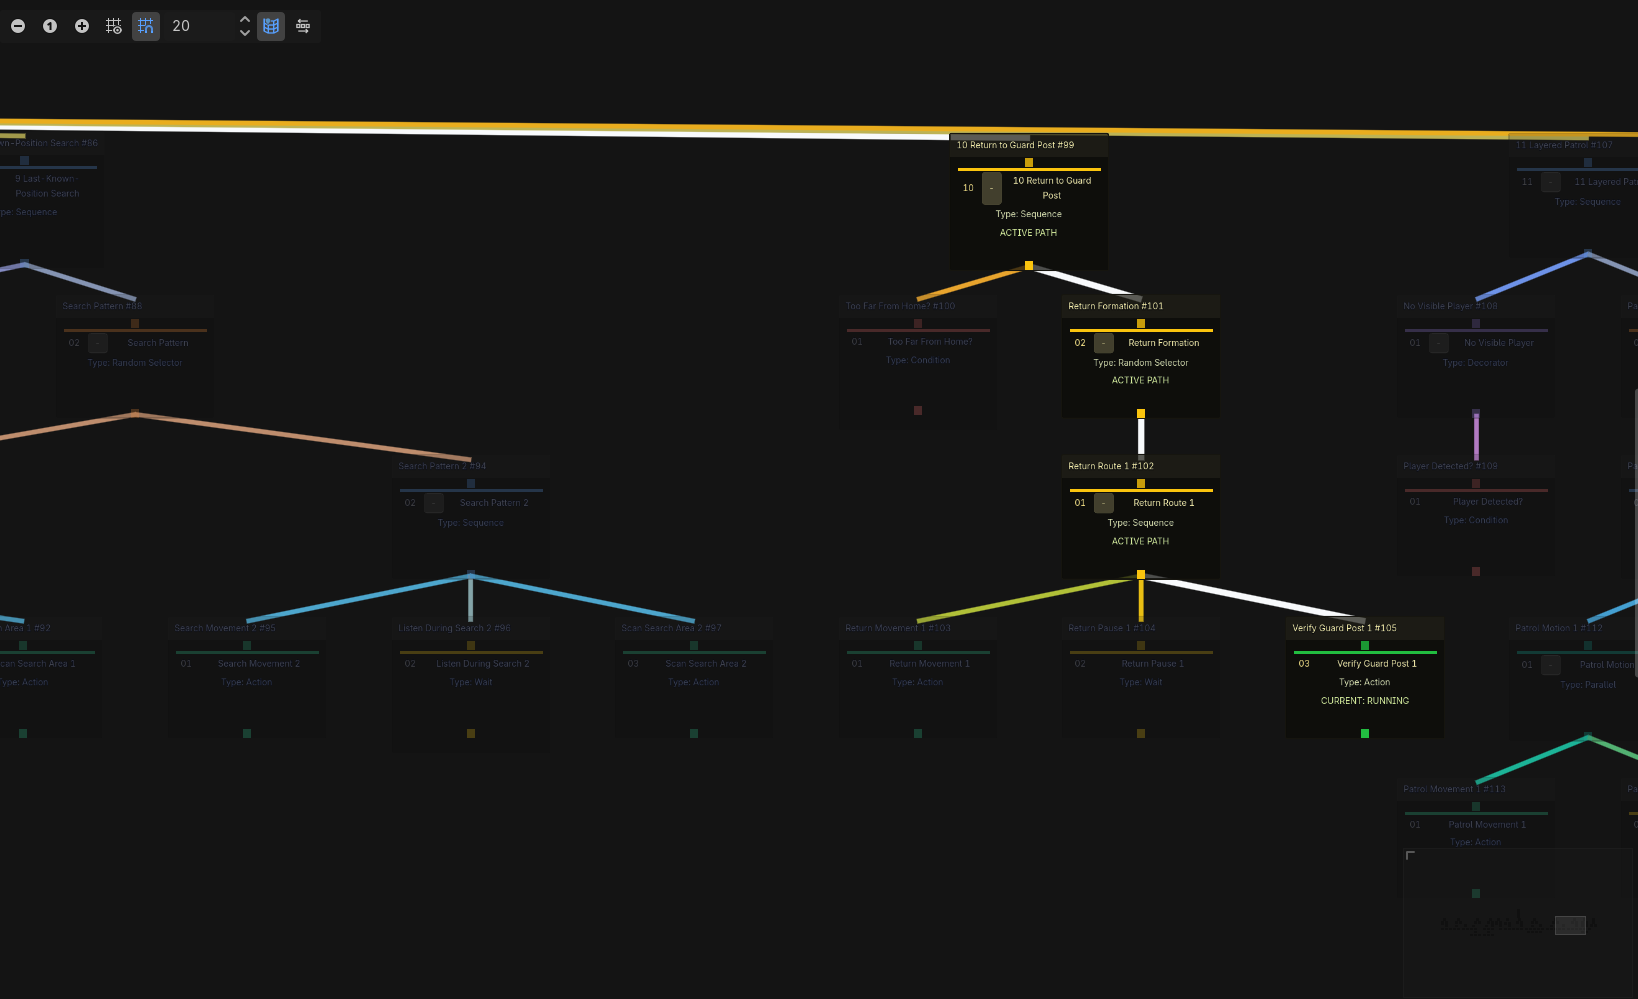
\includegraphics[width=0.92\textwidth,height=0.72\textheight,keepaspectratio]{figures/livedebug.png}
\caption{Live Debug shown on the current 241-node real behaviour tree}
\label{fig:live-debug}
\end{figure}

\section{Display optimisation functions}

\subsection{Smart Drag Reflow}

Smart Drag Reflow is used to solve new occlusion caused by "one node being dragged onto another node". The system starts only after accumulated movement reaches 10 screen pixels, and then updates once every 8 screen pixels of movement. Clicking and very small corrections do not trigger relayout. During dragging, the system directly updates temporary avoidance, so the user can see other cards move away before releasing the mouse.

The algorithm first finds the local structure colliding with the dragged card, and then moves related parent nodes, sibling nodes and children within continuous 2 to 4 layers as a group. At most 24 cards are processed at one time, and the number of collision propagations is limited. This reduces the situation where the whole tree suddenly becomes arranged into regular rows. It only maintains the parent-above-child relationship that was already true before dragging. If the user deliberately placed a group of nodes upside down, the system does not force correction. During single-node dragging, Smart Drag automatically moves nearby cards to reduce occlusion caused by dragging. After the mouse is released, the new position of the dragged node is saved. The position changes of other cards for avoidance only affect the screen display and do not modify the coordinates saved in the behaviour tree. After this function is disabled, these cards return to their original saved positions. When the canvas is rebuilt, the system recalculates whether avoidance is needed according to the currently saved coordinates. After multiple nodes are selected by box selection, the selected nodes move and save as one whole, so their original relative relationship is preserved.

\subsection{Adaptive Zoom Detail}

Adaptive Zoom Detail connects card size and field count to GraphEdit zoom at the same time. When zoom is below 0.62, compact cards of about 188 x 88 are used, and only low detail needed to identify structure is kept. Between 0.62 and 0.88, normal size and medium fields are restored. After reaching 0.88, normal cards of about 250 x 150 and full fields are displayed.

After card size changes, the system rechecks collision on the whole canvas and uses temporary offsets to keep the original relative structure as much as possible. It does not permanently change the tree into another layout, and it is not the local solver of Smart Drag. After zooming in, fields and normal size recover, and disabling the function also clears adaptive size and offset.

This function exchanges information density for overview space. Its purpose is not to keep all text readable after zooming out, but to let the user first see the tree shape and branch range, and then zoom in to check parameters when needed. The later experiment records area reduction, field reduction, changes in cards fully inside the viewport, and hierarchy relationships.

\subsection{Readable Edge Overlay}

Readable Edge Overlay handles local cases where connections are blocked by non-endpoint cards. After it is enabled, the background opacity of supported cards is multiplied by 0.72, so the straight line behind the card can be partly shown. Text, icons and controls use fixed foreground colours and add a 2 px dark outline, so the revealed connection does not pass directly through glyphs. When disabled, the original background, text style and modulation colour are restored.

\subsection{Related Node Focus}

Related Node Focus calculates structural relationships after the user selects nodes. The currently selected nodes use a white border. All their ancestors and descendants use a yellow border. Other nodes under the same parent use a green border. All remaining nodes and connections are clearly dimmed.

When the user needs to select multiple nodes, they can drag a selection box on the blank area, and then move or focus them together. Multi-selection focus merges the ancestors, descendants and sibling relationships of all selected nodes. After the selection is cleared, borders and opacity all recover.

\subsection{Fisheye Focus}

Fisheye Focus is mainly used in an already zoomed-out overview. It continuously changes size according to the distance from the node to the pointer centre. The node closest to the centre is enlarged most clearly, and nearby nodes also receive smaller magnification. Nodes outside the main range shrink and dim. The purpose is to let the user see a local area clearly without leaving the overview.

Fisheye only allows the nearest 8 cards to participate in limited local avoidance. Other nodes do not push the whole canvas because the focus becomes larger. The system uses stable reference positions to calculate distance, and buckets focus position and card size, so slight mouse shaking does not relayout every frame. During mouse-wheel zooming, fisheye pauses briefly and then resumes.

This design prioritises keeping the focus and nearby nodes clear, instead of ensuring that the whole tree has no overlap. Stronger magnification may block nearby cards, so the experiment records target magnification and also separately reports new overlap and hierarchy occlusion.

\section{Test game}

The test game assigns the five behaviour trees of different sizes to five enemies. The player needs to use movement, jumping and attack to defeat these enemies one by one. The scene contains ranged attack, melee, obstacles, jumping routes, ladders, healing items and hazard areas. Enemies can patrol, detect the player, chase, search the last position where the player appeared, traverse obstacles, climb, retreat and recover.

\begin{figure}[htbp]
\centering

\includegraphics[width=0.92\textwidth,height=0.72\textheight,keepaspectratio]{figures/figure_003.png}
\caption{Five behaviour tree sizes controlling five enemies in the playable scene}
\label{fig:test-game}
\end{figure}

Smaller trees use fewer branches to complete basic behaviours, while larger trees take on more combat and environmental responses. After all five enemies are defeated, the game enters the end state.
